\chapter{Methods}
I want the framework and method we use to be easy to use and understand, so that it can easily be discussed among clinicians and other people who don't have a statistics or mathematics background. On the same token, I want the methods and theory to be sound from a statistical point of view. For the three parts that we are combining, there are many different theories and implementations to choose from. I aim to pick the ones that optimize ease of understanding and power of results, with the motivating example being cancer survival data. Throughout this section, we will need to make decisions as to what methods and analyses we will use. Whenever a decision is made, I explain why it was chosen, and alternative methods that could also be used. It is my hope that I will provide enough clarity and detail so that the interested reader can intelligently apply these methods to their own data, even if the choice of methods is different than this thesis.
\section{Multiple Imputation}
\label{sec:MI}
It should be clear that multiple imputation is the preferred method to deal with missing data, so our first decision comes as to what paradigm we should impute under. It should be noted that as long as we can produce valid imputations, the choice of method does not matter. However, since the base of our analysis starts with imputation, we need to make sure that we pick a good method. Everything that follows in the analysis is dependent on our imputed data, so it is necessarily the case that poor imputations will lead to poor results be it bias, high variability, or loss in statistical power.
\subsection{Selecting the MI scheme}
There are two main divisions in modern multiple imputation, and they are joint modelling and full conditional specification. Both have their own flaws and advantages. I will describe both, and then explain why full conditional specification is better suited for cancer research.

Before we get in to the imputation models, we need to have a firm understanding of missing data concepts. They take up quite a bit of space to explain, but they are fundamental concepts. I suggest that everyone reads appendix \ref{app:apdx} (even if you are familiar with MI), so that the concepts and symbols that will be used in this paper are understood. 

In joint modelling (JM), we assume that the missing data mechanism is ignorable and that the data can be described by a multivariate distribution specified by the user on the rows (missing data pattern) of the data. Then, we run a sampler that draws imputations from the specified model, and updates model parameters. Since we don't know the true model parameters, we need to estimate them. This is often done by a data augmentation algorithm \cite{VanBuuren2012}.  A pseudocode example will help better clarify the steps, as can be seen in figure \ref{fig:jmexample}, where we are drawing imputations assuming MVN.
\begin{figure}[h!]
  \centering
    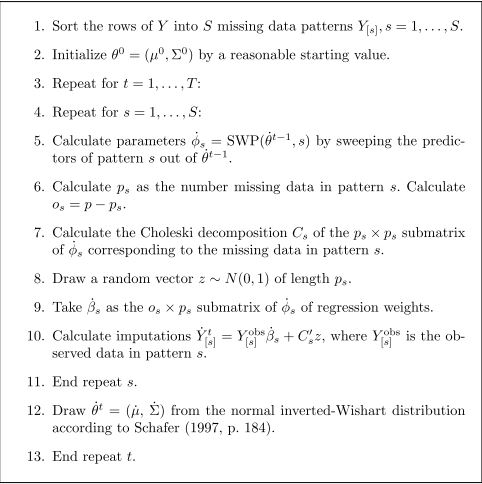
\includegraphics[width=0.8\textwidth]{jm_algo}
  \caption{Normal JM imputation pseudocode}
\label{fig:jmexample}
\medskip
\small
Taken from van Buuren's book �Flexible imputation of missing data� \cite{VanBuuren2012}
\end{figure}

There has been extensive programming and research on using the normal model for this, and research shows that it even performs well under situations where the data has strong non-normality. Some Research has been done for other types of models, but by and large the normal is the most popular. This is just one implementation of a JM approach. Another, like that used in the Amelia package, uses an EM algorithm with user specified priors to make draws.  Other distributions can be used, but the user will have to specify it, derive any relevant distributions, program it, and research the optimality properties.

An obvious issue arises when we have discrete or categorical data (alone or mixed in with continuous). There has been much debate in the literature about what to do with in this case. Some authors argue that you should just impute under a continuous distribution and round imputations to the nearest class number, and others suggest using distributions that are more suited for categorical data \cite{VanBuuren2012}.  < cite here that it is inferior when categorical data present or later?>There are a few of the most used R packages for joint modelling imputation include Amelia \cite{Honaker2015}, norm \cite{norm2015} and cat \cite{cat2015}.

It is my opinion that unless we are very confident in the multivariate joint distribution, that JM should not be used. In our cancer example, we have many categorical variables and strictly positive variables to impute, so JM seems inappropriate.

On the other hand, there is fully conditional specification (FCS). In this paradigm, missing data is imputed on a variable by variable case on the columns/covariates based off of the specification of the imputation model for each covariate, given by the user. Whereas JM imputes on the rows, FCS imputes on the columns. This theory goes by many names, including partially compatible MCMC, iterated univariate imputation, and chained equations \cite{VanBuuren2012}.  These full conditionals should factor to specify the joint distribution. In the JM setting, we must give a k dimensional model, however in the FCS setting, we must give k one dimensional models. We are trying to sample from
%I take out the X's here to keep consistent with the apdx
$$P(Y,R|\theta)$$
By sampling from the full conditionals
$$P(Y_j|Y_{-j},R,\phi_j)$$
In this notation, $Y_-j$ means all of the columns with missing data except for j, and X is the fully observed columns (which could possibly be empty). A pseudocode example can be seen here
\begin{figure}[h!]
  \centering
    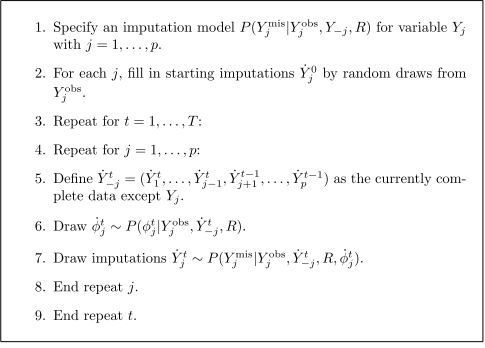
\includegraphics[width=0.8\textwidth]{fcs_algo}
  \caption{Mice FCS imputation pseudocode}
\medskip
\small
Taken from van Buuren's book �Flexible imputation of missing data� \cite{VanBuuren2012}
\end{figure}

One of the major criticisms of this method is that in order for there to be a guarantee that we are sampling from the correct distribution, we need to ensure that our full conditionals are compatible, i.e. that they factor into the proper joint. This is very hard to check in practice, but multiple studies have shown that even when the models are highly incompatible, FCS methods are very robust and produce proper imputations \cite{VanBuuren2006}. FCS allows us much more flexibility than JM does, and it handles discrete and categorical data much better than JM does \cite{Kropko2014}. Some popular R implementations of FCS include MICE \cite{VanBuuren2011}, mi \cite{Su2011}, and BaBooN \cite{Florian2015}. We will be using MICE in the applied section of this paper, and from now on, mice and FCS will be used interchangably.


We are going to have to specify something, there is no escaping that, but I think that it is easier for the average person to be able to define a single distribution and model rather than to guess at a multivariate (which could have a really high dimension). In addition, in the survival analysis setting, we will naturally have time variables be only positive, and some binary indicators, whereas others can take any value. Trying to fit a parametric distribution with these stipulations will be very hard if not impossible, so we will be relegated to using a general distribution (like the normal), which will certainly elicit a poor fit. So, the fully conditional specification certainly seems like the more appealing option.  In an ideal world, we would have complete data, and would not need to resort to imputation. But since we don't have complete data, we must choose one method and accept its strengths and weaknesses.
\begin{comment}
Might want to move elements of this down to application
Now that we have chosen the paradigm, we need to select an implementation of it. Many exist (such as MICE \cite{VanBuuren2011}, mi \cite{Su2011}, etc.). I wanted to select the implementation that combined ease of use, understanding, and programming. What I decided upon was a method called MICE- Multiple Imputation by chained equations \cite{VanBuuren2011} MICE is an FCS MCMC method that under compatibility, is a Gibbs sampler, where we obtain samples from the joint by sampling from the full conditionals. The user defines the full conditionals, so it is possible that the joint may only exist implicitly, and not actually have a functional form. 
\end{comment}

In order to use mice, we must have that the missingness in our data to be MCAR or MAR. It can work with MNAR data, but it requires some extra modelling assumptions. This is a seldom observed case in practice, so the interested reader may check \cite{VanBuuren2011} section 6.2 for a detailed look at this.  Enders proposes using t tests to test if the data is MAR or MCAR, but this is of little use for us, because we only want to know if the data is MNAR, which is impossible to test since testing for MNAR would entail us using information that is impossible to have \cite{Enders2010}. Luckily, we can safely assume MAR if there is reason to believe that some of the covariates collected account for the missingness \cite{VanBuuren2012}.


It should be noted that in the real data we will use, the response variable is fully observed, but the covariates have a lot of missingness. If it were the case that we had missingness in the survival time, then the methods described above might not work. They might fail because the unobserved times may follow a different distribution than the observed times. This is cleared up by Zhao et. al in 2014 through Kaplan-Meier MI  \cite{Zhao2014}. This is beyond the scope of this report though so I omit its details. 
\subsection{Setting and checking the model}
Once we have the correct assumptions, we need to set up our full conditionals imputation models. This may take a while for large datasets, but the extra time spent will ensure a better model. We choose what predictors will go into imputation, and what method to use (regression, predictive mean matching, logistic regression, trees, etc.). We should choose predictor variables that help explain missingness, as well as those we are doing inference on, as to avoid bias \cite{VanBuuren2012}. For variables that are derived from others, we impute the others and then compute that variable, in a process known as passive imputation. Since our data is of manageable size, I include any reasonable predictor that doesn't induce collinearity for predictors in the imputation models. With large datasets, we may need to perform variable selection before specifying the models, so that it doesn't become unmanageable.

Since FCS is an iterative process, we must choose how many iterations we will do until convergence. The older literature suggests only 5 is enough, but with modern computation, we can easily exceed this, even with large data \cite{VanBuuren2012}. A good way to assess how many iterations to run is to look at the diagnostic plots (which we will talk about later), then add 5 iterations to the number at which we assume convergence is achieved. Due to the nature of FCS, convergence is often very quick, often as soon as 5 iterations. As well, we need to decide how many datasets to impute. The early literature argued that 5 would suffice, but modern literature argues for more, since it will cut down on simulation error. Many different authors have different criteria's, but a popular criterion is to impute as many datasets as the 100 times the percentage of cases in the analysis with missingness. With the speed of computers and availability of storage, many authors now suggest using more imputations \cite{VanBuuren2012}.

Once we have determined how many iterations and imputations to run, we actually run mice. Depending on the model specifications, it should not take too long for small datasets (seconds or minutes), but may take a while (hours) for larger ones. FCS models often converges quickly, so after convergence, we are just taking draws from the missing covariates posterior. We can think of the first few iterations as burn in, and the rest as samples. We take the value at the last iteration of each chain as the sample from the posterior.

We need to verify that our imputations are valid once we complete them. First, we need to see if our chains have converged. Since mice is an MCMC method, we should check the chain for irreducibility, aperiodicity, and recurrence. To determine when the chain has converged, van Buuren suggests that ``Convergence is diagnosed when the variance between different sequences is no larger than the variance within each individual sequence'' \cite{VanBuuren2012}.  There is some research (but not from the MI perspective) about tests to check for convergence, and a popular test is Gelman and Rubin's $\hat{R}$ test \cite{Gelman1992}. This test is often used in conjunction with visual tests.  Assessing convergence  by looking at of all of the values over $m$ imputations and $k$ iterations would be very hard to visualize because there would be so many chains, so often times, we will choose to observe a statistic (like the mean) of the chain and assess on that. 

Once we have assessed convergence, we need to actually check that the values imputed are valid and come from the correct posterior. This will serve as our model checking and validation. The overarching idea that we need to pay attention to is �does the data look like it could have been real data�. We can assess this in many ways, including density plots, box and whisker plots, etc. This is a visual task, and there is no statistical method to validate this.

This whole process can be very time consuming, because every time we want to make a change in the methods used, we have to rerun the algorithm and reassess our results. But once we find the setup that works for us, we don't need to repeat it again. So, while it may take a lot of time now, setting up a proper model will save us even more time in the future.

\subsection{Combining the MI estimates}
Once we have $m$ imputed datasets, we may run any valid analysis on each imputed dataset INDIVIDUALLY, treating each of the m datasets as if it was complete. I am a strong advocate of running the model with the available cases if possible before running it on the MI data, so that we can assess the appropriateness of the model. As well, running the model with the available cases will give us a clue as to what to expect from the MI analyses (such as sign of the coefficients or level of significance). 


On the $m$ imputed data sets, we may then apply Rubin's rules \cite{Rubin1987} to pool our estimates. Rubin's rules are essential for using multiply imputed datasets, so we need to investigate them thoroughly. 



Rubin's rules are a set of rules that guide us in making inference from multiply imputed data. They will give us a single point estimate, as well as the proper variance for the quantity we have in mind from the $m$ imputed datasets.  

Rubin's rules involve three parts. The first is getting an estimate of the population estimand Q. To get this, we define $\hat{Q}_i$ as the estimand evaluated from the data in the $i^{th}$ dataset.  Then, we take the average over all $m$ datasets to get a single estimate $\bar{Q}$.
$$\bar{Q}=\frac{1}{m}\sum_{i=1}^{m}\hat{Q}_i$$
The estimates are not set, and there is variance associated with them. The first form of variance is the ``within '' variance, or the variance or each estimate. If we define the variance of the $i^{th}$ imputed dataset as $\bar{U}_i$ , then the overall within variance is computed as
$$\bar{U}=\frac{1}{m}\sum_{i=1}^{m}\bar{U}_i$$


The last form of the variance is the ``between datasets'' variance. This is the variance associated with the fact that we have missing data. It is given by
$$B=\frac{1}{m-1}\sum_{i=1}^{m}(\hat{Q}_i-\bar{Q})$$
The total variance for our estimand is given by 
$$T=\bar{U}+B +\frac{B}{M}$$
The last term is our simulation variance, and its existence is proven by Rubin in \cite{Rubin1987}.

The theory of inference with Rubin's rules is rooted in the assumption that under repeated sampling, the complete data quantity of interest that we are trying to pool is asymptotically normally distributed with mean Q and variance U, where U is the variance $of (Q-\hat{Q})$ \cite{VanBuuren2012}. We don't have the true population variance, so we must use what we have from the sample, namely $T$, the MI total variance. With this assumption, we know that
$$\frac{Q-\bar{Q}}{\sqrt{T}}\sim t_{\nu}$$ 
And the degrees of freedom is proven to be 
$$\nu=\frac{\nu_{old}\nu_{obs}}{\nu_{old}+\nu_{obs}}$$
Where $\nu_{obs}=\frac{\nu_{com}+1}{\nu_{com}+3}\nu_{com}(1-\frac{B + B/m}{T})$
and $\nu_{old}=\frac{m-1}{(\frac{B + B/m}{T})^2}$ \cite{Barnard1999}.

Rubin's rules assume normality, so if our statistic in mind is not asymptotically normal, we need to transform it towards normality before we pool. There have been some research about how to pool non normal quantities, but current research shows poor results and power when doing so \cite{Marshall2009}. It should also be noted that we have discussed the univariate case, but this easily extends the case with multivariate estimands. If we have multivariate estimands, we can still use Rubin's rules, but will need to replace the notation above with vectors for $\hat{Q}_i$ and variance-covariance matrices wherever we have variance. We now have a powerful framework to get valid inference from data with missingness via multiple imputation multiply imputed data, so let's now see how to fit in other types of analyses in the MI paradigm

\section{Survival analysis}
\label{sec:Surv}
Now that we have the multiple imputation datasets created, we may run our analysis on each of them. As a general rule of thumb, we should run our desired analyses on the original data to get the available case estimates, to get an idea of what to expect and to check if the model assumptions are met. Because we are working with cancer data, we are interested in some basic survival quantities, such as Kaplan-Meier survival estimates, log rank test to test for similarity of curves, and Cox regression. Following Rubin's rules, we run the individual analyses on each of the $m$ datasets, and then pool our results. In this section we will discuss each type of survival analysis in the MI setting and the issues associated with it.

At the beginning of the last section, we learned about Rubin's rules, but before we begin, it should be noted that there is another way to work with the multiply imputed data. This method is colloquially called the �stack method�. For the stack method, we take all of our imputed data and �stack� them one on top of each other to get one huge dataset of size $(m*i)$ rows and j columns. Under the stacked method, we can produce unbiased estimates of quantities of interest, but the estimates of variance will be too small (since we are artificially increasing the sample size) \cite{VanBuuren2012}. Thus, the stacked method is a poor choice for running any hypothesis tests or quantifying uncertainty. It is not useless though. The stacked method is useful when we want to analyze just one plot instead of $m$ for model checking. As well, the stacked method may be useful in situations where we partition categorical data on an imputed variable and then look at the percentage in each category. Under the averaging portion of Rubin's rules, we are not guaranteed that the percentages will sum to unity, but under the stacked method we are.

\subsection{Kaplan-Meier Survival Curve}
Analysis for the Kaplan-Meier estimate is quite simply in the non MI setting, but special care should be taken in the MI setting. First, we need to do is clearly define what the groups and population are, and what constitutes an event of interest. A very common mistake that researchers make is to try to frame a competing risks problem as a Kaplan-Meier problem. We also need to be sure that we have noninformative censoring (knowing that the individual is censored tells us nothing about their survival probability). Once we have checked all of these, we can compute the Kaplan-Meier curve on each of the $m$ datasets. For simplicity, in this section we  assume that we run the Kaplan-Meier curve on a dataset with only subjects who take a treatment or a control. Now, we could pool these estimates, but that would be ill advised, because the Kaplan-Meier curve is not normally distributed. To get around this, it has been proposed by Marshall et. al to take the complimentary log log transformation of the survival estimates before pooling \cite{Marshall2009}. We can make this transformation, pool our results, and then back transform to get the pooled KM estimate. 

In the MI setting, an interesting situation may arise when the last event (and thus the range of survival time) differs between the imputed datasets. This is the result of a person with a long survival time being put in different groups via imputation. We can deal with this by either extending the last observed Kaplan-Meier estimate out until the last event time, or truncating all of the imputed curves at the minimum time of last event. In traditional analysis, we would not extend out the Kaplan-Meier curve out past the last event, but if we have wildly varying imputations, this might be a good option, so that we can make inference between curves and are not hampered by one poor imputed dataset.
\subsection{Median Survival Time}
One of the main tasks that clinicians are interested in is the median survival time of each group (the smallest time that the survival function for the group is less than 0.5). The median is the preferred method of central tendency in survival analysis because often times the survival times are right skewed, making the mean a poor estimator of the truth. Finding the median in the MI case is quite simple, as we just take the first time that the averaged Kaplan-Meier curve crosses below 0.5. We would also like to have the variance at the median. The first way to obtain it is to pool the Greenwood variance associated with each time point and then take the average as the variance at that time point. But the Greenwood estimator tends to underestimate the true variance \cite{Klein1984}, and taking the mean of the variance doesn't make much sense. A better solution for this issue is to derive the variance of the median by the ``reflection method''. In this method, we first fit the MI Kaplan Meier curve, and then construct a 95\% confidence interval for all time points using the total variance obtained from Rubin's rules pooling. The median is defined as the first time when the pooled MI curve crosses 0.5 survival line, and the lower and upper bounds are the points where the lower and upper bands cross the .5 survival line respectively. This method is preferred because it uses the variance we actually have, and is much more robust to poor imputations.


\subsection{Log Rank Test}
Now, we will have a pooled estimate of the true survival curve for each group. In the typical setting, we might want to look to see if these curves are similar to each other, so we can determine if the treatment really prolongs survival time. We would do this with a log rank test under the regular setting. However, we should not be deceived. We have an averaged survival curve, they are not constructed in the same way that a regular Kaplan-Meier curve is, so we cannot get the quantities that we would need to compute the log rank test. However, we can still get the pooled log rank test. To do so, we can do one of two things. The first is to run the log rank test on each of the datasets and then pool the results via Rubin's rules. This is the logical way to do it, but under this scheme we will run into a multiple comparison problem. In addition, many statistical packages only report the chi square version of the statistic, meaning we would have to reprogram it in order to use Rubin's rules for pooling. Another option is to run a Cox regression on just the group in question (since this is equivalent to the log rank test under no tied times) \cite{Klein1984}. From the Cox regression, we can obtain the score test. However, in order to do this, we need to know who is in the risk set. But the concept of a risk set doesn't exist in the MI setting. Luckily, we know that the Wald test is asymptotically equivalent to the score test, and the Wald test is very easy to obtain.  So we can use the Wald test of the coefficient from the Cox model as a proxy for the log rank test. In this way, we get a statistic that calculates what we want, while still making sense in the MI context.
\subsection{Cox Proportional Hazards Model}
We would now like to investigate the hazard ratio of different baseline covariates and treatments via the Cox proportional hazards model. The overall goal will be to fit a Cox model with baseline covariates, check to see if it passes the proportional hazards assumption, and then add in the treatment variables to see how they affect the hazard. It is known that the Cox regression coefficients are normally distributed, so there is no issue in pooling, but we do need to be careful about checking the proportional hazards assumption. The very first thing that we need to do is check to check the available case model to assess if we have proportional hazards. If one of the covariates truly is dependent on time, adding imputed data isn't going to change that, so checking the available case analysis is a good sanity check. The way we go about checking to make sure that we have proportional hazards is checking to see if the Schoenfeld residuals are uncorrelated with time for each covariate in the Cox model. The Schoenfeld residuals are tedious to explain and derive, and add no value to this thesis. But knowing that they are partial residuals that that are formulated to be independent of time should suffice to understand this paper \cite{Klein1984}.  We can check a test for correlation or observe a spline fit to the residuals to determine how uncorrelated they are, but the latter is usually preferred in practice. In cancer research, the most common test to look for proportional hazards is to plot the spline fit (often cubic) to the residuals along with the 95\% confidence intervals, and see if any straight line could pass through the bounds. Because the residuals are independent of time, a straight line over time signifies that the hazards are proportional \cite{Schoenfeld1982}. There isn't an official name for this method, but the straight edge method seems to be a fitting name since you can check it by placing a straight edge between the confidence bands.  If this is the case, then we say that that the covariate in question follows the proportional hazards assumption.

We have discussed how to check the proportional hazards assumption in the available case scheme, but how can we do this in the MI setting? We can take our imputed data and fit a Cox model on each of the $m$ datasets, and pool them easily. But how is the best way to check the proportional hazards assumption. We can go about this in a few different ways. The first is to check the assumptions on each individual model fit to each dataset. This may prove to be an arduous task (especially with large $m$, but with graphical tools such as shiny, this isn't too bad). We could also superimpose all of the spline fits on one plot, and see how the shape and general trend compare to the available case analysis. We can also use the stack data to get just one set of plots, but the straight edge method will not work here since the errors are too low. Rather, we would just need to assess the shape of the spline fit in comparison to the available case method.

 Once we have verified that the model follows the proportional hazard assumption, we may trust its results. We can now add in our treatment covariates, and analyze to see how they affect the hazards. An interesting thing to look at will be how the hazards change from the baseline once we factor in the treatment.

\section{Propensity Score Analysis}
\label{sec:Propscore}
Now that we have laid down the theory for analyzing the survival section for clinical relevance, we can move on to the causal analysis part. While there is a lot of preparatory work that goes into the theory of it, the results that can be obtained using causal analysis framework and propensity scores is much stronger and appealing than conventional analysis.  As well, with causal analysis, we get a cause and effect result, which is in tune with what the general population believes that results should be. Propensity score methods are an easy to understand yet powerful tool. The use of propensity scores justified in Rosenbaum and Rubin's 1983 paper \cite{Rosenbaum1983}.   Our overall goal is to estimate the average treatment effect in a setting where the initial study was not an RCT. Propensity score analysis helps us to do this by balancing the groups out so that it becomes more like an RCT.

We will need to make a few decisions along the way. Our very first decision comes when deciding how to use the propensity score. There are four main uses in the survival literature: Matching, stratification, weighting, and covariate adjustment \cite{Austin2014}. The goal is to balance the treatment and control groups, such that the only difference between the groups is due to the treatment received, and not any underlying factor. All of these methods will help us to examine the average causal effect, but each goes about it in a different way. Covariate adjustment and matching have fallen out of favor in the literature recently, but weighting and stratification remain very popular. We will be using weighting in our real data analysis, but I want to first spend some time discussing matching because of its popularity in practice.

If we choose to match propensity scores in the multiple imputation setting, we will need to decide how. The stacking method described before would obviously be inappropriate, as we would have spurious and repetitive matches due the falsely inflated sample size.  Matching on the stacked set would give us much more power to detect a difference, but the results from it would not be valid.

There is hope though for matching with multiple imputation data. Two methods are described in Mitra and Reiter about how to do this \cite{Mitra2012}. In the first method, propensity score matching is done within each MI dataset (known as within matching). Thus, we will get $m$ estimates of the average treatment effect to which we will average. The other method, known as the across method takes the average propensity score for each individual among the $m$ imputed data sets, matches on the averaged propensity scores, and estimates the treatment effect in that manner. Both methods have their pros and cons, and are appropriate for different scenarios. However, the treatment variable may itself have missingness, and thus needs to be imputed. In this situation averaging across datasets does not make sense (since there is no guarantee that a given subject in imputation $i$ has the same treatment in imputation $j$), so we cannot determine if the subject is a case of a control, thus matching will be impossible. When this is the case, we must use the within method. 
%does the fact that the drug is an imputed value effect which model we should use? The problem exists %that the treatment is unknown in some, so it needs to be imputed.  Thus, we could have 30 datasets %where subject I is treatment, and 20 where he is a control. We can either classify as treatment via %majority voting. If not this, then we need to change to the within method.
Propensity scoring using logistic regression is the most widely used method, because it is computationally simple and is well understood by both clinicians and statisticians. Thus, we will use it to compute our propensity scores.

Different propensity scores will be obtained according to what predictors we use in our model, so we need to be sure that we fit a model with clinically relevant and meaningful predictors. Our overarching goal is to account for any pretreatment covariate that leads to the selection of the treatment. There has been significant debate among statisticians about how to set up these models, by either throwing in every possible variable into it, or only include ones known to affect treatment selection. 
%A point to stress is that these all need to be pretreatment variables, because controlling for a covariate %after treatment doesn't make sense. 
I don't plan to settle this debate, but since we are in a setting where simplicity is a goal, I plan to use only pretreatment covariates deemed to be important (through consultation with subject matter experts) to treatment selection. This is the method that Peter Austin (a well-known researcher of propensity score analysis) recommends \cite{Austin2014}. There exists research on how to test if we have properly set up the propensity score model, however, It is not clear how this could be applied in the multiple imputation setting \cite{Li2013}. We should however, check that we have balance between the groups, by examining the standard bias between the groups and looking at balancing tables.
\begin{comment}
The matching can be done in many different ways like a nearest neighbor, caliper, or mahalanobis distance matching. It shouldn't really matter which one we use, so long as the groups are similar in distribution after matching in each dataset.
\end{comment}


Once an acceptable propensity score model is selected, we will need to pick what type of weighting we will do. Many exist, but the most popular are X,Y,Z . We will then run our Cox model again (as in the survival section), but we will factor in the weights. Then, the results that we receive can be viewed  as if they were from a RCT. As well, we can go ahead and analyze them as such, and draw causal inference. I need a lot more work here.

